% This text is proprietary.
% It's a part of presentation made by myself.
% It may not used commercial.
% The noncommercial use such as private and study is free
% Sep. 2010
% Author: Sascha Frank 
% University Freiburg 
% www.informatik.uni-freiburg.de/~frank/
%
% 

\documentclass[handout]{beamer}
\setbeamertemplate{navigation symbols}{}


\usetheme{Warsaw}
\usepackage{ngerman}
\usepackage{media9}
\usepackage[utf8]{inputenc}
\beamersetuncovermixins{\opaqueness<1>{25}}{\opaqueness<2->{15}}
\begin{document}
\title{LES RESEAUX DOMESTIQUES (R. D.)}  
\author{LAVIER Antoine et NTUMBA wa NTUMBA Patient}
\date{\today} 

\begin{frame}
\titlepage
\end{frame} 

\begin{frame}
\frametitle{Contenu}
\tableofcontents
\end{frame} 




\section{Introduction}
\begin{frame}\frametitle{A propos du R. D.} 
Partager sa connexion à Internet, ses fichiers, son imprimante, c'est le rôle essentiel du réseau domestique. Il s'appuie sur le réseau informatique, protocole IP, pour véhiculer n'importe quel type de données numériques, qu'il s'agisse de fichiers ou issus d'Internet.
\end{frame}
\section{Les appareils du réseau domestique}
\begin{frame}\frametitle{Les appareils du R. D.} 
\begin{figure}
		\centering
		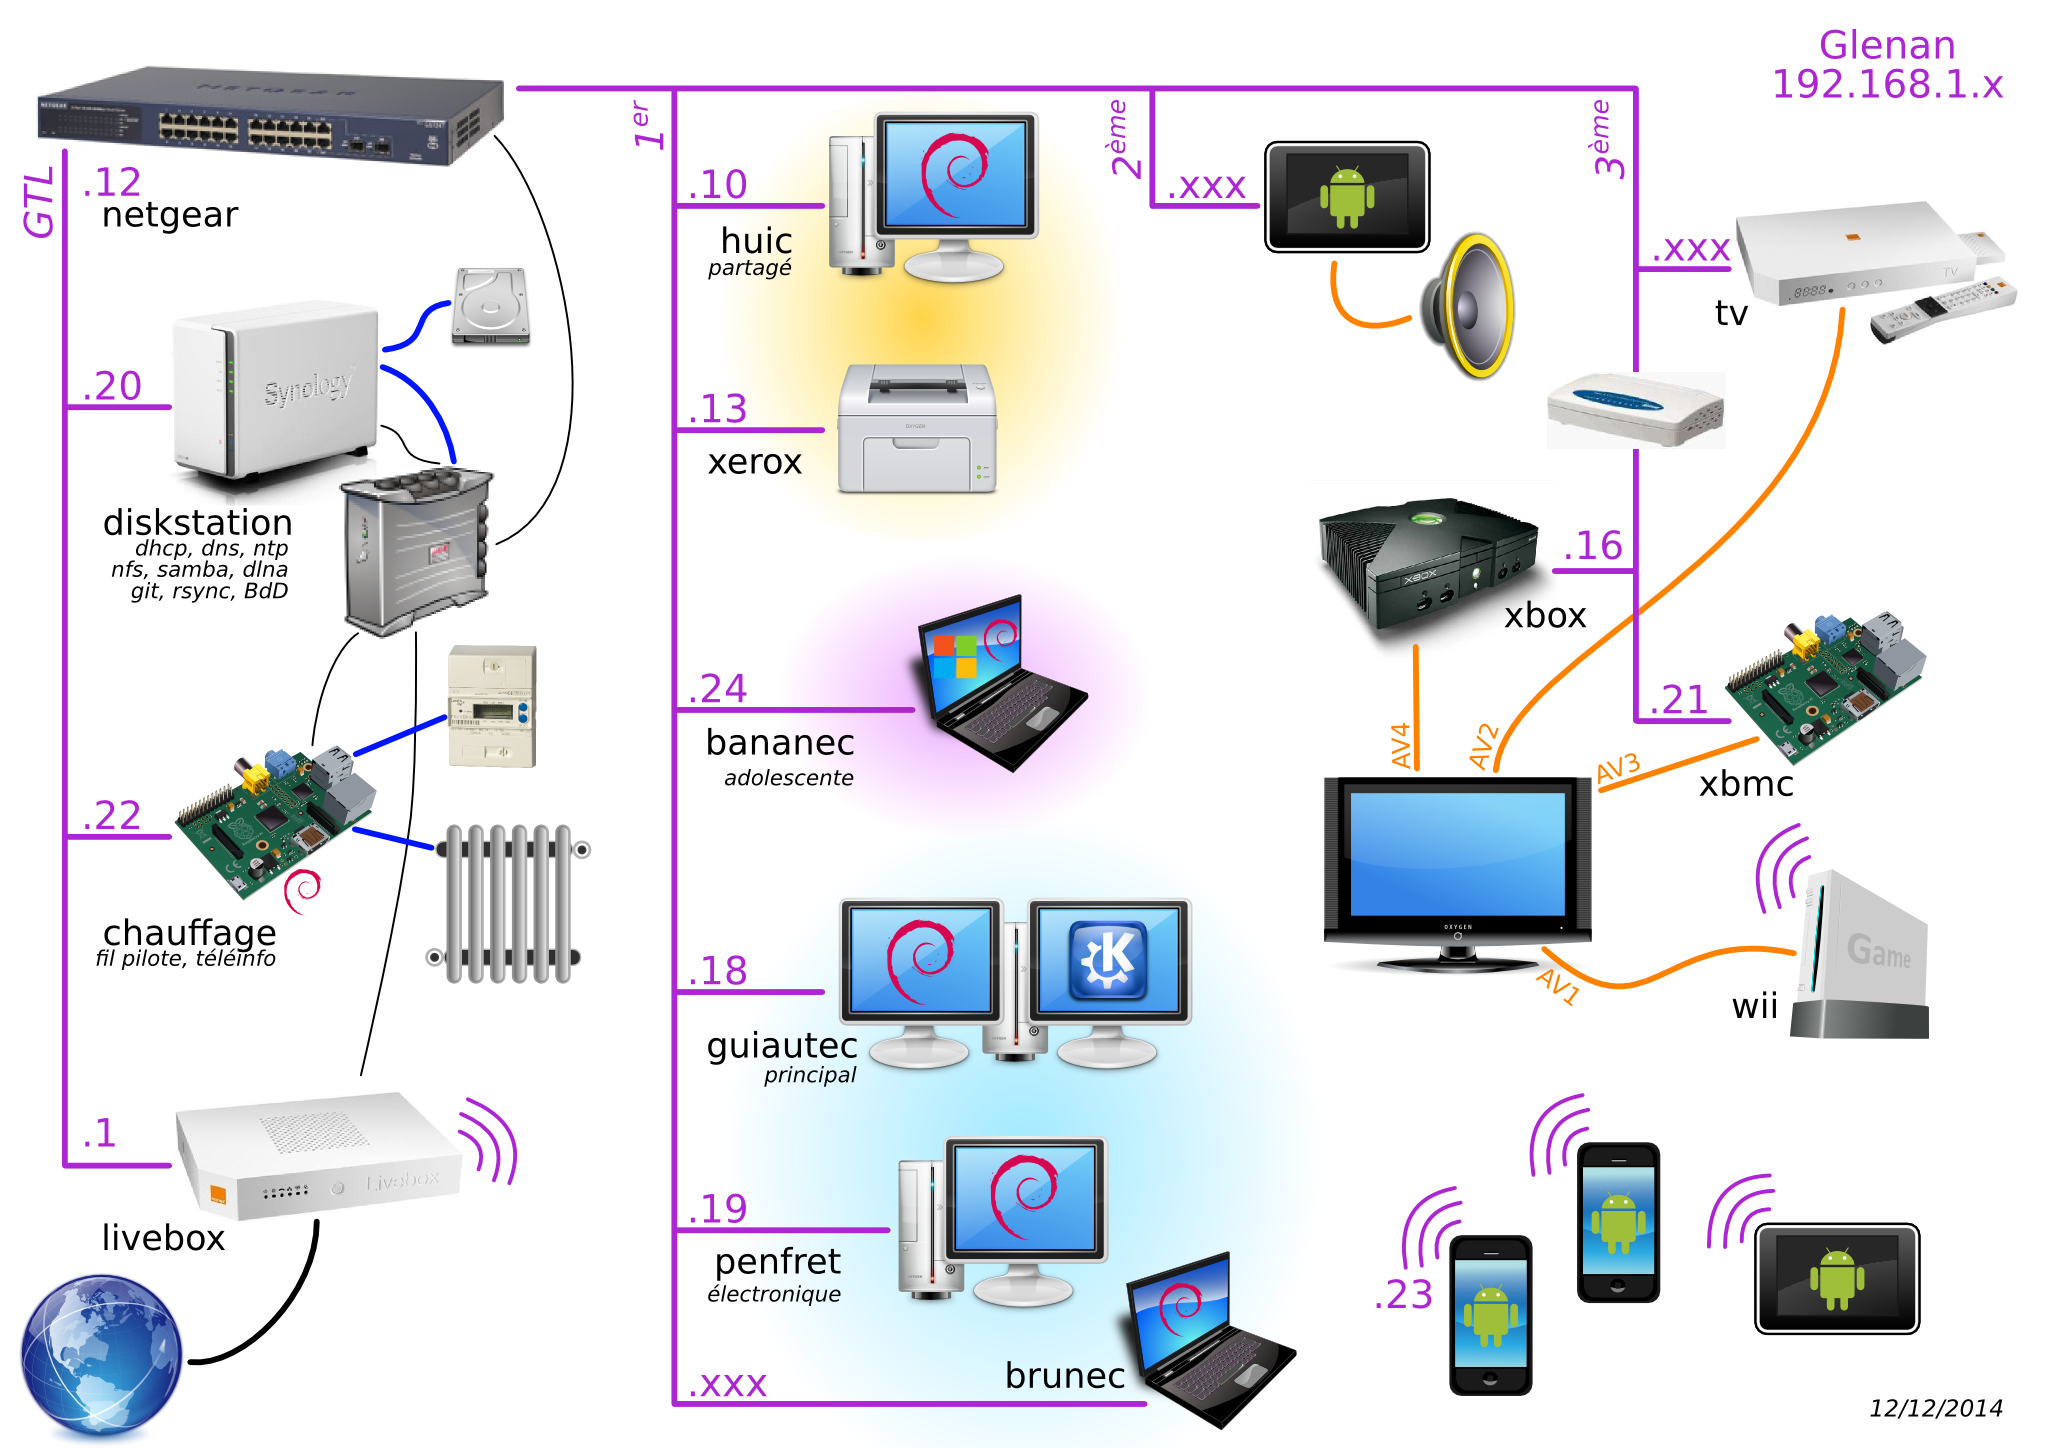
\includegraphics[width=0.8\textwidth,natwidth=100,natheight=100]{image/LAN6.png}
		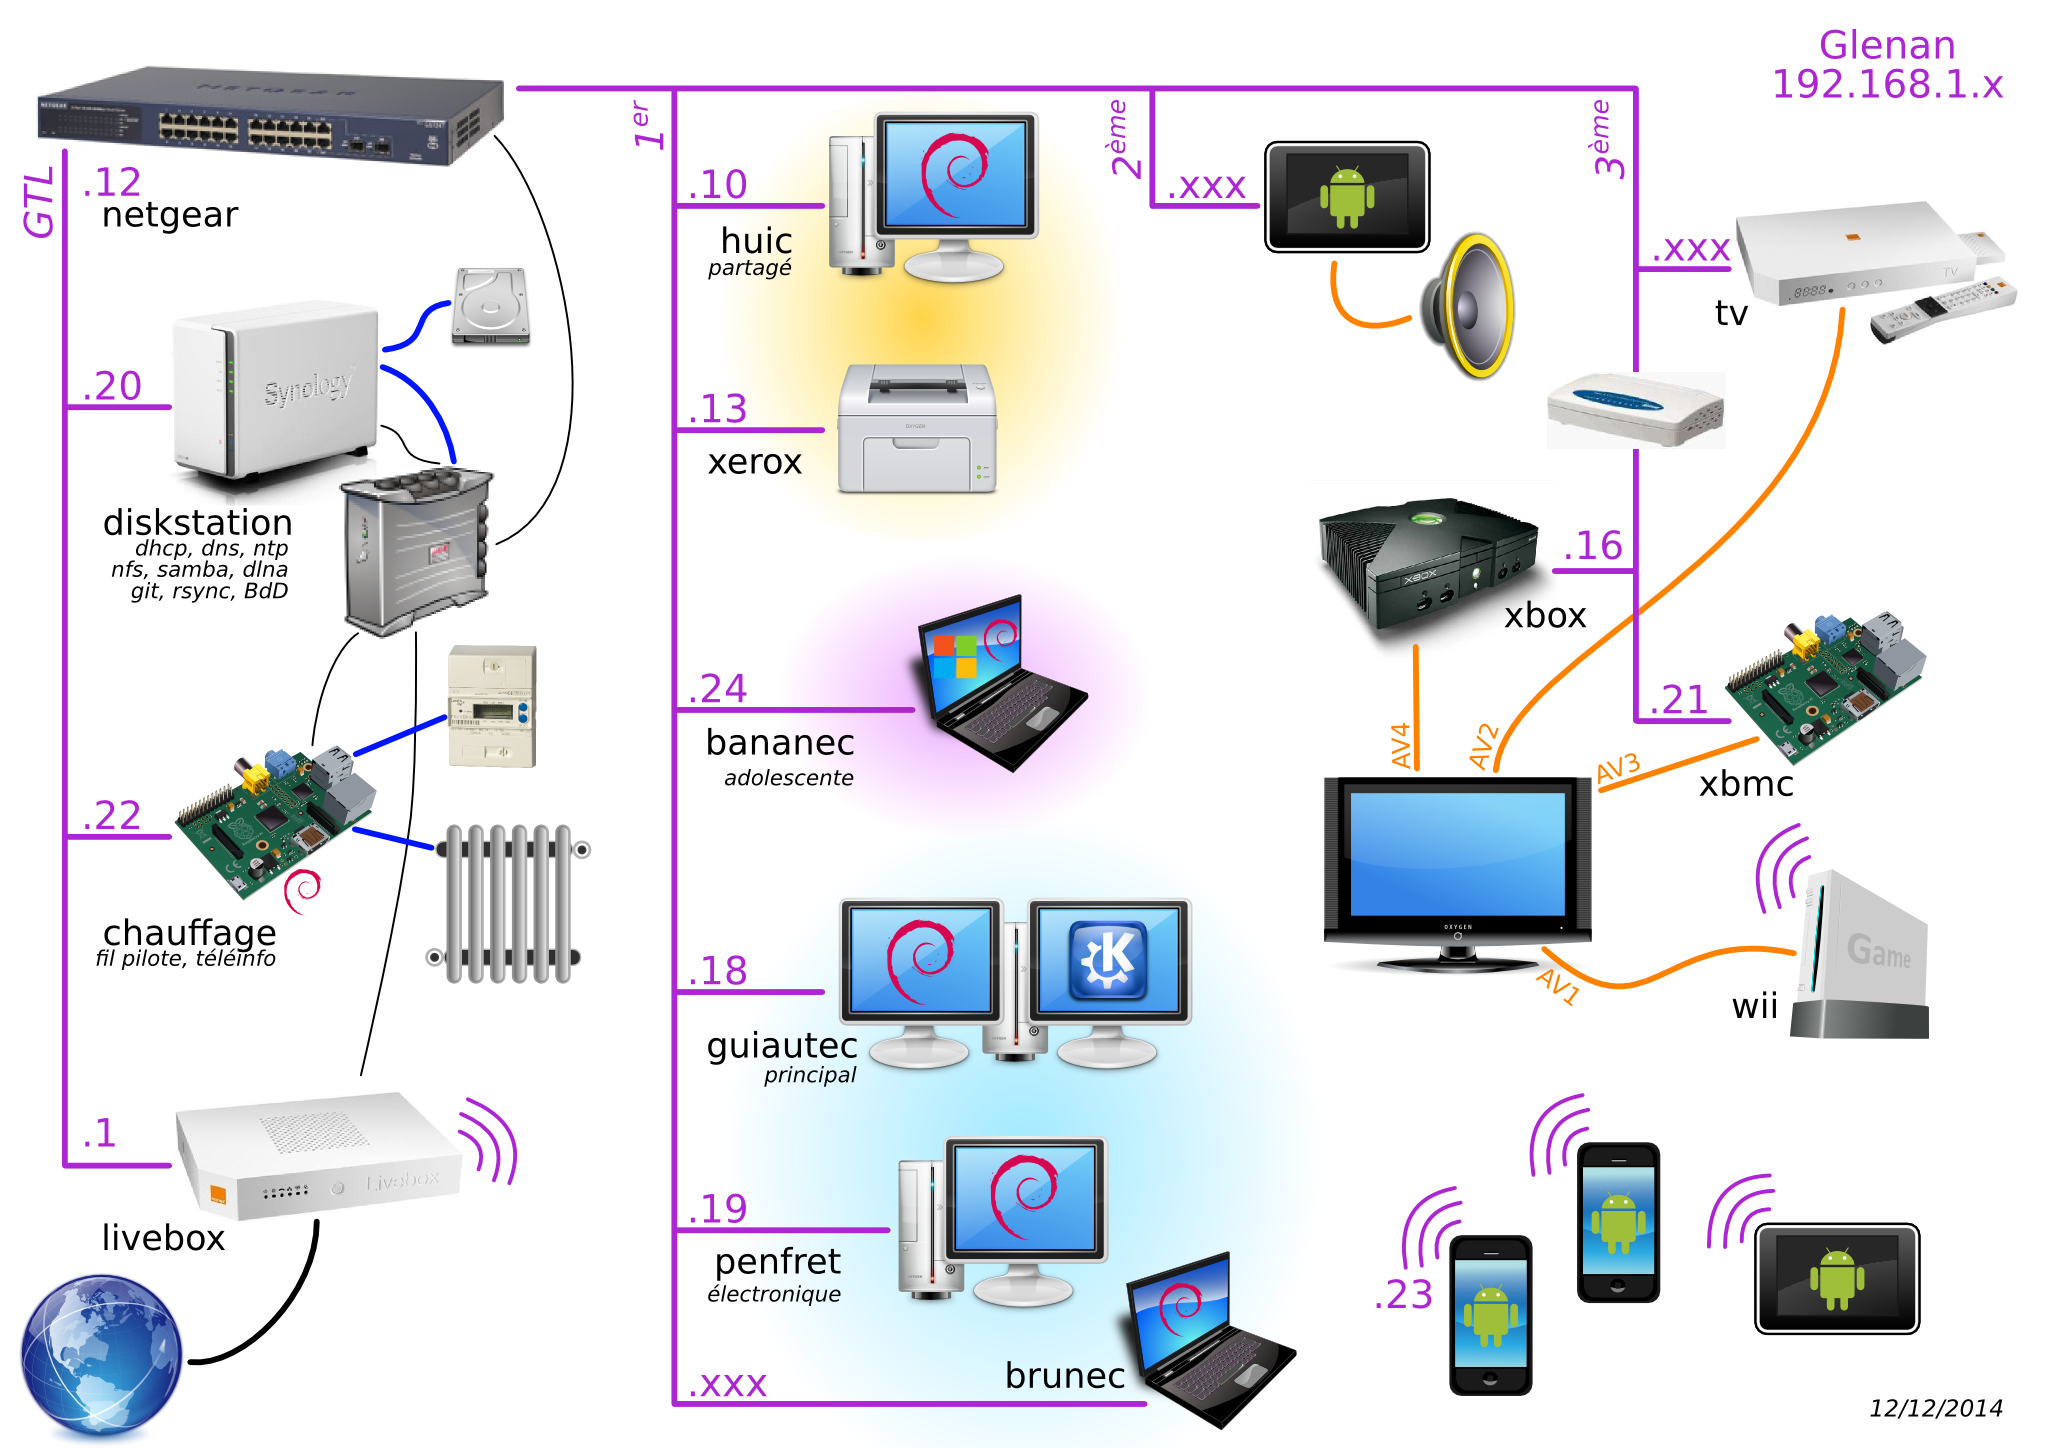
\includegraphics[width=\textwidth,height=0.8\textheight,keepaspectratio]{image/LAN6.png}
\end{figure}
\end{frame}

\section{Insfrastructure}
\begin{frame}\frametitle{Les différents types de liaison} 
\begin{itemize}
\item Ethernet
\item Wifi
\item CPL
\end{itemize}
\end{frame}

\begin{frame}\frametitle{Comparaison des types liaisons} 
\begin{itemize}
\item Portée : Ethernet meilleur que WIFI et CPL
\item Securité : Ethernet et CPL mieux que WIFI
\item Performance
\end{itemize}
\begin{figure}
		\centering
		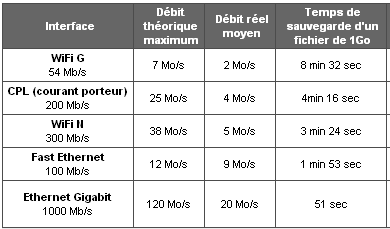
\includegraphics[width=0.5\textwidth,natwidth=100,natheight=100]{image/performance.png}
\end{figure}
\end{frame}

\begin{frame}\frametitle{Les passerelles dans les R. D.} 
\begin{itemize}
\item Les switchs et les hubs
\item Les routeurs et box internet
\item Les points d'accès Wifi
\end{itemize}
\end{frame}

\section{Les services dans un R. D.}
\begin{frame}\frametitle{A la base } 
A la base :
\begin{itemize}
\item Partager sa connexion internet sur différents PC de la maison (box internet) 
\item Partager ses fichiers (NAS)
\item Partager son imprimante
\item Jouer à plusieurs sur un jeu call of dutty
\end{itemize}
\end{frame}

\begin{frame}\frametitle{Différents protocoles / standards associés} 
\begin{itemize}
\item NFS
\item DLNA
\end{itemize}
\end{frame}

\begin{frame}\frametitle{Les besoins de nos jours dans les R.D.} 
\begin{figure}
		\centering
		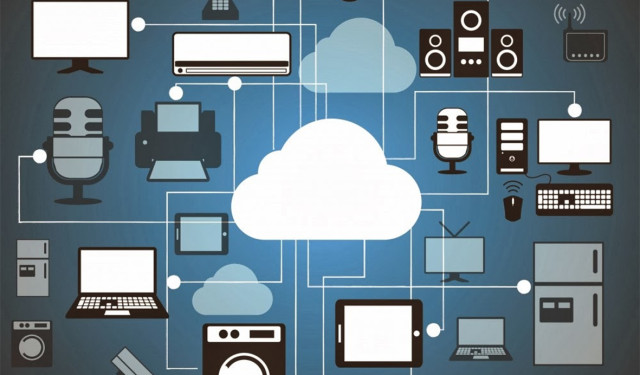
\includegraphics[width=0.5\textwidth,natwidth=100,natheight=100]{image/domotique.jpg}
\end{figure}
\end{frame}

\section{Les objets connectés dans le R. D. ou domotique }
\begin{frame}\frametitle{Un petit mot sur la domotique} 
\begin{figure}
		\centering
		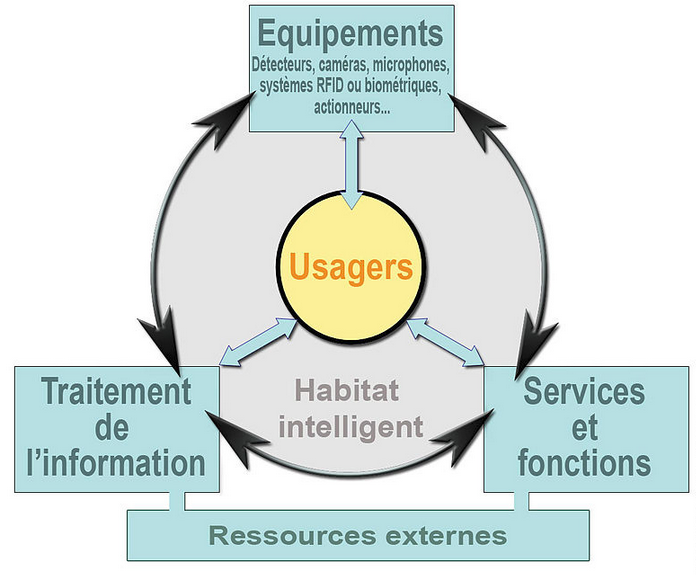
\includegraphics[width=0.5\textwidth,natwidth=100,natheight=100]{image/domotique.png}
\end{figure}
\end{frame}

\begin{frame}\frametitle{Les composants dans la domotique} 
\begin{itemize}
\item  Des surfaces de contrôle avec boutons et/ou télécommandes ;
\item Des systèmes écran et souris, avec clavier avec ou sans fils existent ;
\item  Des interfaces tactiles : écrans tactiles  associés à un logiciel ou une interface web ;
\item Des microphones permettent une activation par commande vocale,  directement ou via GSM, VoIP, associés à des logiciels de reconnaissance vocale ;
\item Des logiciel de reconnaissance des gestes, d'empreinte digitale
\end{itemize}
\end{frame}


\begin{frame}\frametitle{Mode de transmission des données} 
\begin{itemize}
\item Par Onde radio hertzienne : comme le Bluetooth, IO-HomeControle, zigbee, X2D, KNX, Wireless USB;
\item Par infrarouge
\item Par réseau cablé : comme Ethernet, EIB/Konnex, SCS BUS / OpenWebNet, USB, LonWorks, UPnP, RS485;
\end{itemize}
\end{frame}

\begin{frame}\frametitle{Mode de transmission des données} 
\begin{itemize}
\item Combien coute l'installation de la domotique
\linebreak
Dans une construction d’une maison neuve de taille comprise entre 130 à 170 m2 , le cout de la domotique répresente entre 4 et 10 pourcent du coup global de la construction, soit 8 000 Euro et 20 000 Euro pour une maison de 200 000 Euro
\linebreak
\item Normalisation de l'installation, La norme NFC 15-100 et le guide UTE C 90-483
\end{itemize}
\end{frame}

\section{Et la maison du futur}
\begin{frame}\frametitle{SmartHome 3.0} 
 https://www.youtube.com/watch?v=TptZ8m8prd4
\begin{figure}
    \centering
    \includemedia[
    width=0.6\linewidth,height=0.3375\linewidth,
    activate=pageopen,
    flashvars={
        modestbranding=1 % no YT logo in control bar
        &autohide=1 % controlbar autohide
        &showinfo=0 % no title and other info before start
        &rel=0 % no related videos after end
    }
        ]{}{https://www.youtube.com/watch?v=TptZ8m8prd4}
\end{figure}
\end{frame}
\end{document}
